% 第9章第2节：泛函的最优条件（无约束一阶条件、约束一阶条件、二阶条件）。

\section{泛函的最优条件}
\label{sec:opt-fn-optimality}

上一节只回答了“扰动之后目标怎样变化”。现在假定候选函数与所需微分都已给定，反过来问：若$u^\star$是最小点，这些变化必须满足什么条件？必要条件按允许的扰动方向逐一建立，充分条件则要求额外的结构。有限维中的同类结论见第~\ref{chap:optimization}章；本节说明哪些论证可以照搬，哪些在无限维中需要加强。

\subsection{无约束一阶条件}
\label{sec:opt-fn-unconstrained-first}

最小点附近，沿任何一条直线看过去，目标都不能下降。这一观察把函数空间中的问题化为一元函数的极值问题。

\begin{theorem}[一阶必要条件]
\label{thm:opt-fn-first-order-necessary}
设$J$在$u^\star$的某个开邻域$U$内取有限值，$u^\star$是$J$的局部最小点，即$J(u^\star)\le J(u)$对$U$中所有$u$成立。若$J$在$u^\star$处Gâteaux可微，则
\[
 DJ(u^\star)[h]=0\qquad\text{对所有}h\in X .
\]
在Hilbert空间中，这等价于$\nabla_HJ(u^\star)=0$。
\end{theorem}

\begin{proof}
固定$h$，令$\varphi(t)=J(u^\star+th)$。$|t|$足够小时$u^\star+th\in U$，所以$\varphi(t)\ge\varphi(0)$。$t>0$时差商$(\varphi(t)-\varphi(0))/t\ge0$，$t<0$时差商$\le0$；两侧极限都等于$DJ(u^\star)[h]$，故它既非负又非正，只能为零。
\end{proof}

证明只比较了$h$与$-h$两个方向上的一维变化，没有用到微分的线性。定理的前提是最小点存在；它只是筛选候选的条件，不能说明满足$DJ(u)=0$的$u$是最小点，也不能说明这样的$u$存在。

\paragraph{凸性给出充分性}
对凸目标，零微分已经足够。设$X$中的凸集$K$上$J$取有限值且凸，即对$u,v\in K$、$t\in[0,1]$有$J(u+t(v-u))\le(1-t)J(u)+tJ(v)$；凸函数及其一阶刻画的有限维版本见第~\ref{chap:optimization}章。若$J$在$K$的内点$u$处Gâteaux可微，则对每个$v\in K$，
\[
 \frac{J(u+t(v-u))-J(u)}t\le J(v)-J(u),\qquad0<t\le1 ;
\]
令$t\to0^+$，左边趋于$DJ(u)[v-u]$，得到一阶支撑不等式
\begin{equation}
 J(v)\ge J(u)+DJ(u)[v-u]\qquad\text{对所有}v\in K .
 \label{eq:opt-fn-convex-support}
\end{equation}
若$DJ(u^\star)=0$，则$J(v)\ge J(u^\star)$对所有$v\in K$成立，$u^\star$是$K$上的全局最小点。

\paragraph{驻点可以不是最小点}
在$X=L^2(0,1)$上取$J_1(u)=-\bigl(\int_0^1u\,dx\bigr)^2$与$J_2(u)=\bigl(\int_0^1u\,dx\bigr)^3$。两者在$u=0$处的微分都是零：$J_1(th)=-t^2(\int h)^2$，$J_2(th)=t^3(\int h)^3$，除以$t$后都趋于零。限制到常函数$u\equiv c$上，它们分别是$-c^2$和$c^3$，零点分别是最大点和没有极值的点。零微分方程“解出来了”并不意味着找到了最小点，从必要条件到充分条件需要凸性或下面的二阶条件这样的额外结构。

\subsection{约束一阶条件}
\label{sec:opt-fn-constrained-first}

候选受约束时，$u^\star+th$可能离开可行集，上一小节的双向比较不再可用。我们先看哪些扰动保持可行，再在这些方向上重复同样的论证。

\paragraph{仿射约束：在方向空间上为零}
章首的固定端点问题中，可行集$C=\{u\in H^1(0,1):u(0)=0,u(1)=1\}$是仿射集：任取$u_0\in C$（例如$u_0(x)=x$），则$C=u_0+V$，其中$V=\{h\in H^1(0,1):h(0)=h(1)=0\}=H_0^1(0,1)$。对$u\in C$与$h\in V$，$u+th$对所有实数$t$都可行，可以作正负两个方向的扰动。均值约束$\int_0^1u\,dx=m$同样给出仿射集，方向空间是$\{h:\int_0^1h\,dx=0\}$。

\begin{theorem}[仿射约束下的一阶必要条件]
\label{thm:opt-fn-affine-first-order}
设$C=u_0+V$，$V$是$X$的线性子空间，$J$在$u^\star\in C$的某个开邻域内取有限值且在$u^\star$处Gâteaux可微。若$u^\star$是$J$在$C$上的局部最小点，则$DJ(u^\star)[h]=0$对所有$h\in V$成立。
\end{theorem}

证明与定理~\ref{thm:opt-fn-first-order-necessary}相同，只是$h$限于$V$。结论只约束微分在$V$上的作用，不要求整个微分为零。固定端点问题中，最优点满足$\int_0^1u^{\star\prime}h'\,dx=0$对所有$h\in H_0^1(0,1)$成立，而不是对所有$h\in H^1(0,1)$：取$h\equiv1$时$\int u^{\star\prime}\cdot0=0$自然成立，取$h(x)=x$则一般不为零，这个方向会破坏端点条件，不在允许之列。

\paragraph{凸约束：变分不等式}
可行集是凸集但不是仿射集时，只能沿指向集合内部的线段移动。设$C$凸，$u^\star\in C$，$v\in C$，则线段$u^\star+t(v-u^\star)$，$t\in[0,1]$，留在$C$中。

\begin{theorem}[凸约束下的一阶条件]
\label{thm:opt-fn-variational-inequality}
设$C\subseteq X$凸，$J$在$u^\star\in C$的某个开邻域内取有限值且在$u^\star$处Gâteaux可微。
\begin{enumerate}
 \item 若$u^\star$是$J$在$C$上的局部最小点，则
 \begin{equation}
  DJ(u^\star)[v-u^\star]\ge0\qquad\text{对所有}v\in C .
  \label{eq:opt-fn-variational-inequality}
 \end{equation}
 \item 若$J$在一个包含$C$的凸集上凸，则~\eqref{eq:opt-fn-variational-inequality}推出$u^\star$是$J$在$C$上的全局最小点。
\end{enumerate}
\end{theorem}

\begin{proof}
(1) 令$\varphi(t)=J(u^\star+t(v-u^\star))$。$t>0$足够小时$\varphi(t)\ge\varphi(0)$，所以单侧差商非负，其极限$DJ(u^\star)[v-u^\star]\ge0$。(2) 由支撑不等式~\eqref{eq:opt-fn-convex-support}，$J(v)\ge J(u^\star)+DJ(u^\star)[v-u^\star]\ge J(u^\star)$。
\end{proof}

形如~\eqref{eq:opt-fn-variational-inequality}的条件称为\term{变分不等式}（variational inequality）。它只要求微分在指向可行集的方向上非负，边界上的最小点不必使整个空间的梯度为零。

\begin{example}[非负约束下的最近函数]
\label{ex:opt-fn-positivity}
在$X=L^2(0,1)$中取$g(x)=\sin(2\pi x)$，在$C=\{u\in L^2(0,1):u\ge0\text{ 几乎处处}\}$上最小化$J(u)=\frac12\int_0^1(u-g)^2dx$。$C$凸，$J$凸且$\nabla_{L^2}J(u)=u-g$。候选$u^\star=\max(g,0)$满足变分不等式：$u^\star-g=\max(-g,0)$只在$u^\star=0$的地方不为零，于是对任意$v\in C$，
\[
 \int_0^1(u^\star-g)(v-u^\star)\,dx=\int_{\{g<0\}}(-g)\,v\,dx\ge0 .
\]
由定理~\ref{thm:opt-fn-variational-inequality}(2)，$u^\star$是全局最小点，最小值为$\frac12\int_{\{g<0\}}g^2dx=1/8$。图~\ref{fig:opt-fn-positivity-vi}中，梯度$u^\star-g$（黄）在后半区间明显不为零，它“想把”$u$往下推，但那里$u^\star$已贴着约束$u\ge0$，任何可行方向$v-u^\star$在该处都非负，内积因而非负。
\end{example}

\begin{figure}[!htb]
  \centering
  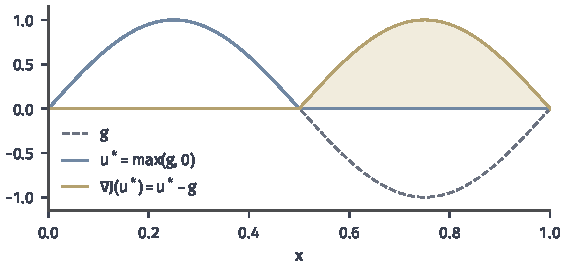
\includegraphics[width=96mm]{figures/03-optimization-evolution-and-signals/01-optimization/matplotlib/c9-positivity-vi/figure.pdf}
  \caption{非负约束下的最优函数。灰色虚线为$g(x)=\sin(2\pi x)$，蓝线为最优解$u^\star=\max(g,0)$（图中记作$u^*$），黄线及浅黄区域为梯度$u^\star-g=\max(-g,0)$。梯度只在$u^\star=0$处非零，并且指向约束之外，满足变分不等式而不等于零。}
  \label{fig:opt-fn-positivity-vi}
\end{figure}

\paragraph{非凸约束}
若$C$不凸，$u^\star$与$v\in C$之间的线段可能离开$C$，变分不等式的推导失效。这时需要重新描述可行方向，例如沿留在$C$中的曲线$t\mapsto c(t)$求导；等式约束$\|u\|_H=1$这样的球面就属于此类，其处理方式与第~\ref{chap:constrained-optimization}章中有限维的切方向和KKT条件相同，本章不再展开。

\subsection{二阶条件}
\label{sec:opt-fn-second-order}

一阶条件无法区分最小点与最大点。和有限维一样，下一步看二阶项；无限维中的新问题在于“正定”需要一个统一的下界。

\paragraph{二阶展开}
设$J$在$u$的开邻域内有限，若存在有界线性泛函$DJ(u)$与有界对称双线性形式$D^2J(u):X\times X\to\mathbb R$，使
\begin{equation}
 J(u+h)=J(u)+DJ(u)[h]+\tfrac12D^2J(u)[h,h]+o(\|h\|_X^2) ,
 \label{eq:opt-fn-second-expansion}
\end{equation}
就说$J$在$u$处有二阶展开。例如平方误差$E(u)=\frac12(Lu-y)^2$的展开是精确的，$D^2E(u)[h,h]=(Lh)^2$；$J_0$的二阶项是$\int_0^1h'^2dx$。

\begin{theorem}[二阶条件]
\label{thm:opt-fn-second-order}
设$C=u^\star+V$，$V$为线性子空间（$V=X$即无约束情形），$J$在$u^\star$处有二阶展开~\eqref{eq:opt-fn-second-expansion}。
\begin{enumerate}
 \item 若$u^\star$是$J$在$C$上的局部最小点，则对所有$h\in V$，都有$DJ(u^\star)[h]=0$，并且$D^2J(u^\star)[h,h]\ge0$。
 \item 若对所有$h\in V$都有$DJ(u^\star)[h]=0$，并且存在常数$c>0$，使所有$h\in V$满足$D^2J(u^\star)[h,h]\ge c\|h\|_X^2$，则存在$\rho>0$，使$h\in V$、$\|h\|_X<\rho$时
 \[
  J(u^\star+h)\ge J(u^\star)+\tfrac c4\|h\|_X^2 .
 \]
 特别地，$u^\star$是$C$上的严格局部最小点。
\end{enumerate}
\end{theorem}

\begin{proof}
(1) 一阶部分即定理~\ref{thm:opt-fn-affine-first-order}。固定$h\in V$，$t\to0$时$0\le J(u^\star+th)-J(u^\star)=\frac{t^2}2D^2J(u^\star)[h,h]+o(t^2)$，两边除以$t^2$再取极限即得。(2) 取$\rho$使$\|h\|_X<\rho$时余项绝对值不超过$\frac c4\|h\|_X^2$，则$J(u^\star+h)-J(u^\star)\ge\frac c2\|h\|_X^2-\frac c4\|h\|_X^2$。
\end{proof}

必要条件只要求二阶项半正定，充分条件要求一致的正下界$c$。一般非线性约束下的二阶判别还涉及约束本身的曲率与临界方向，不能只看目标的二阶项，本节不讨论。

\paragraph{每个方向为正，仍可能不是最小点}
有限维中，二次型在每个非零方向上为正就推出存在共同的$c>0$，因为单位球面是紧集。无限维中单位球面不紧，这一步失败。在$\ell^2$上取
\[
 J(\bm x)=\sum_{k=1}^\infty\frac{x_k^2}k-\sum_{k=1}^\infty x_k^4 .
\]
由$\sum_kx_k^4\le(\sum_kx_k^2)^2=\|\bm x\|_2^4$，第二项是$o(\|\bm x\|_2^2)$，所以$J$在原点的二阶展开为$DJ(0)=0$、$D^2J(0)[\bm h,\bm h]=2\sum_kh_k^2/k$，对每个$\bm h\neq0$都为正。但没有共同的$c$：沿第$k$个坐标方向$\bm e_k$，$D^2J(0)[\bm e_k,\bm e_k]=2/k\to0$。原点也确实不是局部最小点：$J(t\bm e_k)=t^2/k-t^4$在$t>1/\sqrt k$时为负，而$1/\sqrt k\to0$，原点的任意小邻域里都有使$J<0=J(0)$的点。图~\ref{fig:opt-fn-no-uniform-curvature}画出这些截线：每条在原点附近都向上弯，但弯曲越来越平，越过零点的位置越来越靠近原点。

\begin{figure}[!htb]
  \centering
  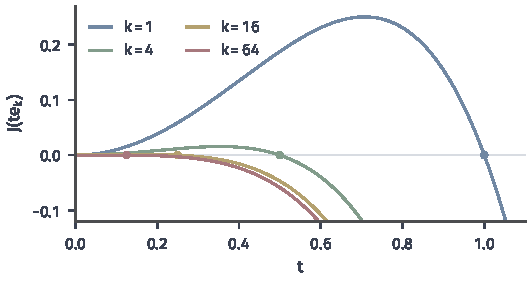
\includegraphics[width=90mm]{figures/03-optimization-evolution-and-signals/01-optimization/matplotlib/c9-no-uniform-curvature/figure.pdf}
  \caption{二阶项逐方向为正但没有一致下界。$\ell^2$上$J(\bm x)=\sum_kx_k^2/k-\sum_kx_k^4$沿坐标方向的截线$J(t\bm e_k)=t^2/k-t^4$，$k=1,4,16,64$；圆点标出零点$t=1/\sqrt k$。原点处每条截线的二阶导数$2/k$都为正，零点却随$k$增大逼近原点。}
  \label{fig:opt-fn-no-uniform-curvature}
\end{figure}
